\documentclass[]{article}

\usepackage[utf8]{inputenc}
\usepackage{amsmath}
\usepackage{amssymb}
\usepackage{amsthm}
\usepackage{amsfonts}
\usepackage{mathtools}
\usepackage[margin=1.7cm]{geometry}
\usepackage[most]{tcolorbox}
\usepackage{graphicx}
\usepackage{capt-of}
\usepackage{adjustbox}
\usepackage{listings}
\usepackage{cleveref}
\usepackage{siunitx}
\usepackage{subcaption}
\usepackage{siunitx}
\usepackage{biblatex}
\addbibresource{sample.bib}
\usepackage[section]{placeins}
\usepackage{float}




% Section numbering %
%\renewcommand\thesection{Assignment \arabic{section}}
%\renewcommand\thesubsection{\arabic{subsection}}

% Proofs
\newcommand\TombStone{\rule{.5em}{.5em}} % The tombest stone
\renewcommand\qedsymbol{\TombStone}
\renewcommand{\proofname}{Proof.} % Nice proof

\title{Interactive Multiple Model Probability Data Association Filter}
\author{Håvard Mellby \& Sigurd Totland}


\begin{document}
\maketitle
\subsection{Abstract}
Sensor Fusion is an important aspect of modern robotics. Any single sensor is never perfect, and the need for fusing together multiple sensors is crucial to allow machines to percieve our world. In this report we will implement three different solutions to three different problems using sensor fusion with a bayesian framework. The implementations performance and consistency will be discusses using common metrics such as NEES and NIS, and we will compare the results from simulations with the results from real world data.
\subsection{Introduction}
The course \texttt{TTK4250 Sensor Fusion} introduces several methods for target tracking, navigation and mapping using a variety of sensors. During the course we have developed a radar tracker for boats using an \texttt{interactive multiple models probability data association filter} and tested it on real world data from the \texttt{Joyride} dataset. We have also created an \texttt{error state kalman filter} tracking the 6 degrees of freedom of an airplane as well as IMU biases using inertial navigation and GNSS. Lastly we have done \texttt{simultanious localization and mapping} using odometry and LIDAR data by implementing an EKF-SLAM approach. In this report we will summarize our approach and findings for all three methods.


%\newpage
\section{}

\subsection{IMM-PDAF}
\subsubsection{IMM}
In target tracking, the behaviour of the targets we want to model might change over time, and any single, reasonably simple model might not cover all situations. A better approach might be to combine multiple simple models with each model describing a subset of the full system behaviour. In our case we want to model a boat that is either moving straight forward or turning. We can then use an \textit{interactive multiple models} (IMM) approach to combine a CT (Constant Turn) and a CV (Constant Velocity) model. The IMM will weigh the different models based on how well they describe the current state using the likelihood of the model being the correct one.

\subsubsection{PDAF}
No sensor is perfect and radars are no exception. The radar outputs a lot of measurements which may or may not originate from our target. To solve this we use a \texttt{probability data association filter} to associate measurements with our target and weigh them according to their likelihood of originating from our target.

We can combine the IMM and PDAF to develop the \texttt{interactive multiple models probability data association filter} to track a moving boat using radar detections.

\subsubsection{Implementation}
A normal IMM filter was developed according to chapter 6 in \cite{edmund} and was initialized with a CT and a CV EKF model. Most of the IMM-PDAF implementation is equal to the PDAF implementation described in chapter 7 in \cite{edmund} using the IMM as the model. There are however one difference that we should emphasize.

When updating the IMM conditional on each possible measurement association we get a new mixture model from the IMM with $M$ components. The total mixture model for the IMM-PDAF after one iteration (assuming single gaussian input) is therefore a mixture model with $(N+1)M$ components where $N$ is the number of gated measurements and $M$ is the number of models. This will again continue to grow for each timestep as new measurements will create additional components.

We therefore want to reduce the number of components by conditioning the association probabilities on the mode probabilities. Further we reduce the mixture for each mode to a single gaussian component using equation (6.18) and (6.20) from \cite{edmund}. The association probabilities conditioned on the mode are used as weights.




\subsection{Tune the IMM-PDAF to the Given Simulated Data}

We initialized the filter using the values from previous exercises which we knew worked well. We then modified the \textit{simulate\_atc\_track.m} script to allow us to generate pure CV and CT tracks and used those to tune the corresponding CV/CT PDAF models, using the NEES $95 \%$ confidence interval (CI) and common sense as metrics. Multiple simulated tracks were used for each model to increase robustness. The measurement noise $r$, clutter intensity $\lambda$, the detection probability $P_D$ and the gate size should be independent of modes, so they were tuned and balanced between the two models. The clutter rate $\lambda$ can be interpreted as the number of false detections per cubic meter and it is therefore reasonable for this number to be quite low. The process noise for CV $q_{cv}$ and CT $q_{ct}$ were tuned individually using their correspondig models. For IMM PDAF tuning we created a custom plot function which allowed us to plot the tracked path in colors corresponding to the mode probability (see \cref{fig:task22_modeprob}). We then tuned the IMM Markov Matrix $\pi$ so that the CV model was used during constant velocity sections of the track, and the CT models during the turns (fig \ref{fig:task22_modeprob_tuned}). $q_{cv}$ and $q_{ct}$ does affect the mode probabilities, i.e we risk always preferring one model if the process noises are not balanced (see fig \ref{fig:task22_modeprob_highcv} where $q_{cv}$ is big compared to $q_{ct}$). Our finished tuning works well and seems to balance the two models well. The NEES is mostly within the $95\%$ CI as can be seen in \cref{fig:task22_NEES}. The estimation error, as shown in \cref{fig:task22_tracking_error}, is also quite small and well within what we consider acceptable limits.

\begin{tcolorbox}[ams align, title={Tuning for IMM-PDAF in simulated dataset}]
        r &= 5 & \lambda &= 10^{-4} \label{eq:imm-sim-tuning1} \\
        P_D &= 0.95 & \texttt{gateSize} &= 5^2 \label{eq:imm-sim-tuning2} \\
        q_{cv} &= 0.0078  & q_{ct} &= \begin{bmatrix}0.02 & 0.0005\end{bmatrix} \label{eq:imm-sim-tuning3} \\
        \Pi &= \begin{bmatrix}0.90 & 0.05 \\ 0.10 & 0.95\end{bmatrix} \label{eq:imm-sim-tuning4}
\end{tcolorbox}

\begin{figure}
    \centering
    \hspace*{-2cm}\begin{adjustbox}{minipage=0.8\linewidth, scale=1}
        \begin{subfigure}{.5\textwidth}
            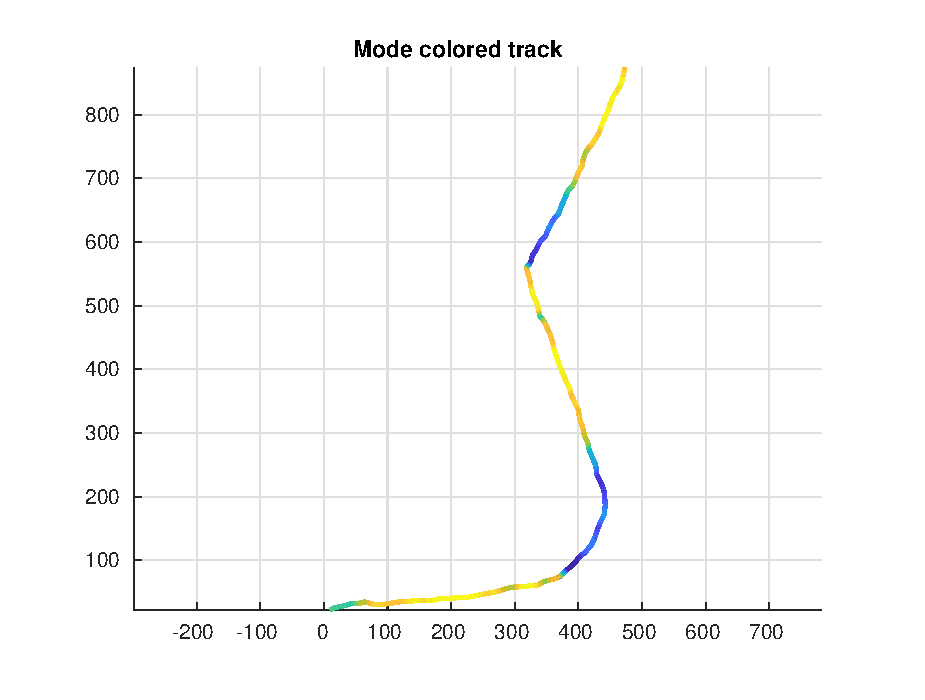
\includegraphics[width=\linewidth]{plots/task22_modeprob.eps}
            \caption{Our tuning}
            \label{fig:task22_modeprob_tuned}
        \end{subfigure}
        \begin{subfigure}{.5\textwidth}
            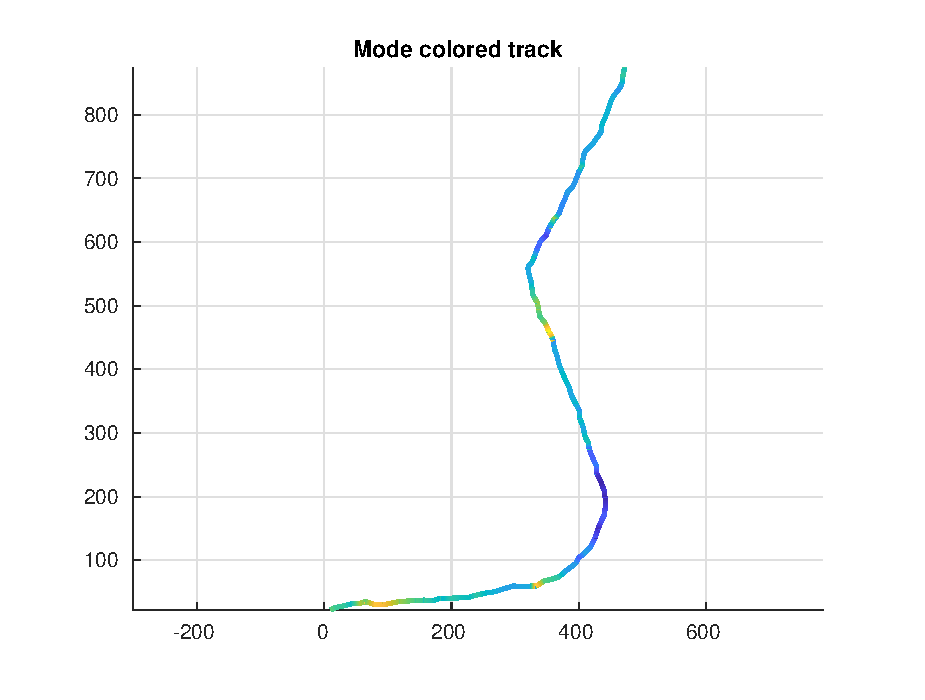
\includegraphics[width=\linewidth]{plots/task22_modeprob_highcv.eps}
            \caption{$q_{cv}$ and $q_{ct}$ not in balance}
            \label{fig:task22_modeprob_highcv}
        \end{subfigure}
    \end{adjustbox}
        \caption{Mode probability plot: Yellow = CV, Blue = CT}
        \label{fig:task22_modeprob}
\end{figure}

\begin{figure}
    \centering
    \hspace*{-2cm}\begin{adjustbox}{minipage=0.8\linewidth, scale=1}
        \begin{subfigure}{.5\textwidth}
            \includegraphics[width=\linewidth]{plots/a1/task2/a1_task2_error.eps}
            \caption{Tracking error}
            \label{fig:task22_tracking_error}
        \end{subfigure}
        \begin{subfigure}{.5\textwidth}
            \includegraphics[width=\linewidth]{plots/a1/task2/a1_task2_NEES.eps}
            \caption{NEES}
            \label{fig:task22_NEES}
        \end{subfigure}
    \end{adjustbox}
        \caption{Tracking performance when using simulated data}
\end{figure}

\subsection{IMM-PDAF on the Real Dataset "Joyride"}
Tuning of IMM-PDAF for the real dataset "joyride" was a bit more tricky. In the simulated dataset there were more distinct sections of either turning or constant velocity. We could also generate independent datasets for tuning each model. On the real dataset we have to model everything at once and it is challenging to get a robust track at all. We initialized the filter using the parameters from task 2 which resulted in loss of track after only a few turns. We introduced a third model $CV_{high}$ (high model noise $q_{CV_{high}}$) which caputures the dynamics not well explained by our CV or CT models. (e.g high linear acceleration). Once we found some values that gave us a complete track we could try an iterative approach to improve NEES and the estimation error. We set an $95\%$ CI for the NEES and tried small variations in all parameters. The clutter rate $\lambda$ and detection probability $P_D$ had to be reduced quite a bit, while the measurement noise $r$ had to be increased to get a robust track. The process noise $q_{CV}$ and $q_{CT}$ also had to be increased quite a bit compared to task 2. When tuning the process noise $q_{CV}$ and $q_{CT}$ as well as the transition probabilities $\pi$ we made sure that there was a clear distinction in the mode probabilities between the CV and CT models. The colored track plot from task 2 was used to visualize when the different modes were preferred by the filter, as shown in \cref{fig:task3_mode_prob_track}. The process noise $q_{CV_{high}}$ was set a lot higher to make sure it was left out unless none of the other models could explain a set of measurements. As seen in \cref{fig:task3_mode_prob_track} it was hardly used at all.
The Markov matrix $\pi$ was tuned to prefer the CV and CT models.
\begin{tcolorbox}[ams align, title={Tuning for IMM-PDAF for "Joyride" dataset}]
        r &= 400 & \lambda &= 5*10^{-6} \label{eq:imm-real-tuning1} \\
        P_D &= 0.85 & \texttt{gateSize} &= 5^2 \label{eq:imm-real-tuning2} \\
        q_{cv} &= 0.1 & q_{cv_{high}} &= 100 \label{eq:imm-real-tuning3} \\
        q_{ct} &= \begin{bmatrix}4 & 0.0000002\end{bmatrix} & \Pi &= \begin{bmatrix}0.90 & 0.05 \\ 0.10 & 0.95\end{bmatrix} \label{eq:imm-real-tuning4}
\end{tcolorbox}
\begin{figure}
    \centering
    \hspace*{-2cm}\begin{adjustbox}{minipage=0.8\linewidth, scale=1}
        \begin{subfigure}{.5\textwidth}
            \includegraphics[width=\linewidth]{plots/a1/task3/a1_task3_error.eps}
            \caption{Tracking error}
            \label{fig:task3_tracking_error}
        \end{subfigure}
        \begin{subfigure}{.5\textwidth}
            \includegraphics[width=\linewidth]{plots/a1/task3/a1_task3_NEES.eps}
            \caption{NEES}
            \label{fig:task3_NEES}
        \end{subfigure}
    \end{adjustbox}
        \caption{Tracking performance when using the real dataset "Joyride"}
\end{figure}

\begin{figure}
    \centering
    \hspace*{-2cm}\begin{adjustbox}{minipage=0.8\linewidth, scale=1}
        \begin{subfigure}{.5\textwidth}
            \includegraphics[width=\linewidth]{plots/a1/task3/a1_task3_tracked_path.eps}
            \caption{Track vs ground truth: BLUE=track, RED=ground truth}
            \label{fig:task3_track}
        \end{subfigure}
        \begin{subfigure}{.5\textwidth}
            \includegraphics[width=\linewidth]{plots/a1/task3/a1_task3_mode_colored_track.eps}
            \caption{Mode probabilities}
            \label{fig:task3_mode_prob_track}
        \end{subfigure}
    \end{adjustbox}
        \caption{Joyride track}
\end{figure}

\subsubsection{Discussion}
We also tested with the much simpler CV and CT PDAF models to compare results. Both the CT and CV EKF PDAF models worked suprisingly well on the dataset and they were much simpler to tune. We even got a higher proportion of NEES within our CI, but with a small increase in tracking error (RMSE). This makes sense since the simpler models are easier to get consistent, but with a loss in tracking precision. 
\section{}
\subsection{ESKF}
The human brain is brilliant filter fusing multiple senses together to create what we percieve. We rely on multiple senses to be able to know if we are falling or to know where we are. 
Robots have the same need when navigating and we do not have any single perfect sensor that can fully provide us with the robots pose at any time. We therefore want to create a filter to fuse multiple sources of data together to create an estimate for our robot, similar to how our brain create our perception.

We will therefore develop the \texttt{error state kalman filter} (ESKF) to estimate the location and orientation of an aeroplane using intertial navigation. The plane use an \texttt{intertial measurement unit} (IMU) to sense acceleration and rotation rate using accelerometer and gyroscope. Similar to a human with his/her eyes closed, the filter is able to predict pose using only the IMU if the prior state is known, but with an increasing error (and corresponding uncertianty). We will therefore also use a GNSS receiver to update our estimate when we receive new measurements. 

A normal EKF, which might be tempting to use, struggles with representing the error state covariance due to the nonlinearity which occurs when working with orientation. We therefore use our measurements to estimate the error state directly. We then use our model to simulate the nominal state using numerical integration methods. After measurement updates we get estimates for the error states which we can inject into our nomial state predictions and correct for any model or simulation errors. After the injection step the error can be reset back to zero and we avoid having to propogate the error. (i.e why keep the error if we "know" what is it?). By doing this we avoid having to find a relationship between the error state covariance and the nominal state covariance (not trivial when working with attitude), since we can get the covariance directly from the ESKF. We can also use different representations for orientation when predicting the nominal state and when estimating the error covariance. 

We also consider the IMU measurement as control input to our model and not as measurements. Measurements would require us to include the acceleration and orientation rates as part of the state vector, and we do not have any good model for these. The computational complexity would also increase due to the high rate of IMU measurements.
\subsection{Tuning of ESKF for simulated data}
We initialized the tuning by looking up typical values for GNASS and IMUs. We tuned $q_a$ and $q_\omega$ according to \cref{sec:using_datasheet}. We tuned the standard deviation for GNASS using \texttt{eskf.NISGNSS} and attempted to get it within the $95\%$ CI. We increased the standard deviation for the altitude component in the GNSS measurement noise since GNSS is usually best at estimating XY position. For the bias models we selected a reciprocal time constant $p_{ab} = p_{\omega b} = 10^{-3}$ after some trial and error. The bias noises were hand tuned to get NEES for bias within the $95\%$ CI. We also looked at the estimation errors and made sure they remained reasonably low. We had extra focus on the attitude error because it propogates into the acceleration in the intertial frame (which causes a lot of errors when integrated twice for position). The error state covariance was initialized to a quite low value to avoid long period of large errors in the beginning until the filter has converged. Initialization is important for ESKF as it can  converge very slow if initialized incorrectly.

\subsubsection{Using parameters from STIM300 datasheet}\label{sec:using_datasheet}
To tune the ESKF acceleration and angular velocity continious time noise we used the STIM300 datasheet \cite{stim300} and used the values for angular random walk (table 6.3 in \cite{stim300}) and velocity random walk (table 6.4 in \cite{stim300}). 
The datasheet specifies angle as degrees, so we had to convert the angular random walk to radians.
The random walk parameters can then be scaled using $h=3600s$ and multiplied by the square root of the IMU rate $\sqrt{\frac{1}{dt}}$ to get the continious time noise parameters $q_a$ and $q_\omega$.


\begin{figure}
    \centering
    \begin{adjustbox}{minipage=1.1\linewidth, scale=1}
        \begin{subfigure}{.5\textwidth}
            \includegraphics[width=\linewidth]{plots/a2-sim-state_error.pdf} 
            \caption{State error}
            \label{fig:a2-sim-state_error}
        \end{subfigure}
        \begin{subfigure}{.5\textwidth}
            \includegraphics[width=\linewidth]{plots/a2-sim-nees.pdf} 
            \caption{NEES}
            \label{fig:a2-sim-nees}
        \end{subfigure}
    \end{adjustbox}
        \caption{ESKF filter error for simulated data}
        \label{fig:a2-sim-error_NEES}
\end{figure}
\begin{figure}
    \centering
    \includegraphics[width=0.7\linewidth]{plots/a2-sim-estimates.pdf} 
    \caption{State estimates}
    \label{fig:a2-sim-estimates}
\end{figure}

\begin{align}
        RGNSS &= (0.29)^2\begin{bmatrix}
    1^2 & 0 & 0 \\
    0 & 1^2 & 0 \\
    0 & 0 & 1.6^2
\end{bmatrix} & q_a &= (1.167 \cdot 10^{-3})^2 * 100Hz \label{eq:eskf-sim-tuning1} \\
        q_{ab} &= (2.2 \cdot 10^{-3})^2 & p_{ab} &= 10^{-3} \label{eq:eskf-sim-tuning2} \\
        q_\omega &= deg2rad((2.5 \cdot 10^{-3})^\circ)^2 * 100Hz  & q_{\omega b} &= (1.2 \cdot 10^{-5})^2 \label{eq:eskf-sim-tuning3} \\
        p_{\omega b} &= 10^{-3} \label{eq:eskf-sim-tuning4}
\end{align}

 

\subsection{Tuning of ESKF for real data} \label{a2task3}
The next step was to see how the error state Kalman filter would perform on actual real life data. The available dataset contains IMU and GNSS measurements of a unmanned aerial vehicle (UAV) remotely controlled by an operator. The flight path of the UAV as seen from the GNSS measurements is shown in figure \ref{fig:real-track}.
\begin{figure}[H]
\centering
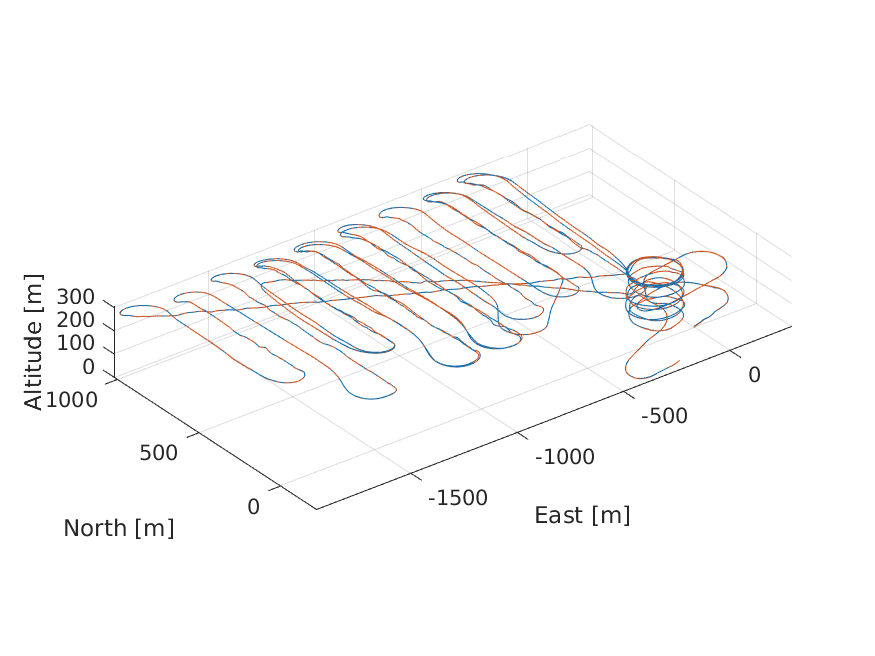
\includegraphics[width=0.6\textwidth]{plots/a2-real-track}
\caption{UAV Track for the real dataset. Red=GNSS measurements, Blue=ESKF}
\label{fig:real-track}
\end{figure}
With this real dataset, there are some other complications that must be adressed. First is the correction matrices $S_a$ and $S_g$ for the gyro and the accelerometer. These matrices correct for the orientation of the IMU in the body frame of the AUV. They also correct for misaligned axes IMU axes (that is, the IMU may be slightly malproduced with axes that are skewed somewhat off the orthogonal coordinate axes). These matrices however are of course not known exactly, because they are supposed to correct for unknown manufacturing errors, for this reason must expect some inaccuracy in the measurements. The second complication is the leverarm. This is the distance between the cener of control on the AUV and the mounting position of the IMU. This value has been measured and is given in the dataset. We give it as an input to the ESKF.

The tuning of the kalman filter model is again based on the STIM300 datasheet, as this is the actual IMU used on the UAV. The acceleration noise $qA$ and gyro noise $qG$ were set by looking up the specification for the IMUs random walk parameters (scaled using $h=3600s$) and use those to find the discrete time noise parameters. Then we used equation 10.70 in \cite{edmund} to scale the noise using our IMU rate of 250Hz. 
\begin{equation}
q_a = (\frac{0.07}{60})^2 * 250Hz = (1.167*10^{-3}*\sqrt{250})^2
\end{equation}
\begin{equation}
q_g = \text{deg2rad}(\frac{0.15}{60})^2 * 250Hz = \text{deg2rad}(2.5*10^{-3}*\sqrt{250})^2
\end{equation}
The gyro noise was also converted to radians. We tuned the bias models by hand, heavily inspired by our tuning from the simulated dataset. In this case, we do not have the ground truth available, so we cannot calculate the normalised error state squared (NEES). We are also not able to tune the filter using the error state. We can however use the \textit{innovation} of the kalman filter, which in layman terms is a measure of how much the filter must update or "innovate" the estimate in the update step to correct for the new measurement. In other words we can measure how "off" the prediction is which we further can compare with how certain the filter is when predicting. We also have the GNSS receivers estimated accuracy which we scaled and used as the standard deviation for the GNSS measurements. With our tuning, we are able to achieve a normalized innovation squared (NIS) that stays $82\%$ inside the $95\%$ $\chi^2$ confidence interval, shown in figure \ref{fig:nis_basic} below. We also split the NIS into one planar and one altitude component due to the difference in accuracy for GNSS. We then used the two NIS metrics when scaling $RGNSS$. We attempted to further tune the IMU noises, but decided it was better to use the official values provided by the manufacturer. Without ground truth and error metrics, it is difficult to further quantify the performance of the filter and therefore difficult to further improve the tuning. 

\begin{figure}[H]
        \centering
        \begin{subfigure}[b]{0.45\textwidth}
                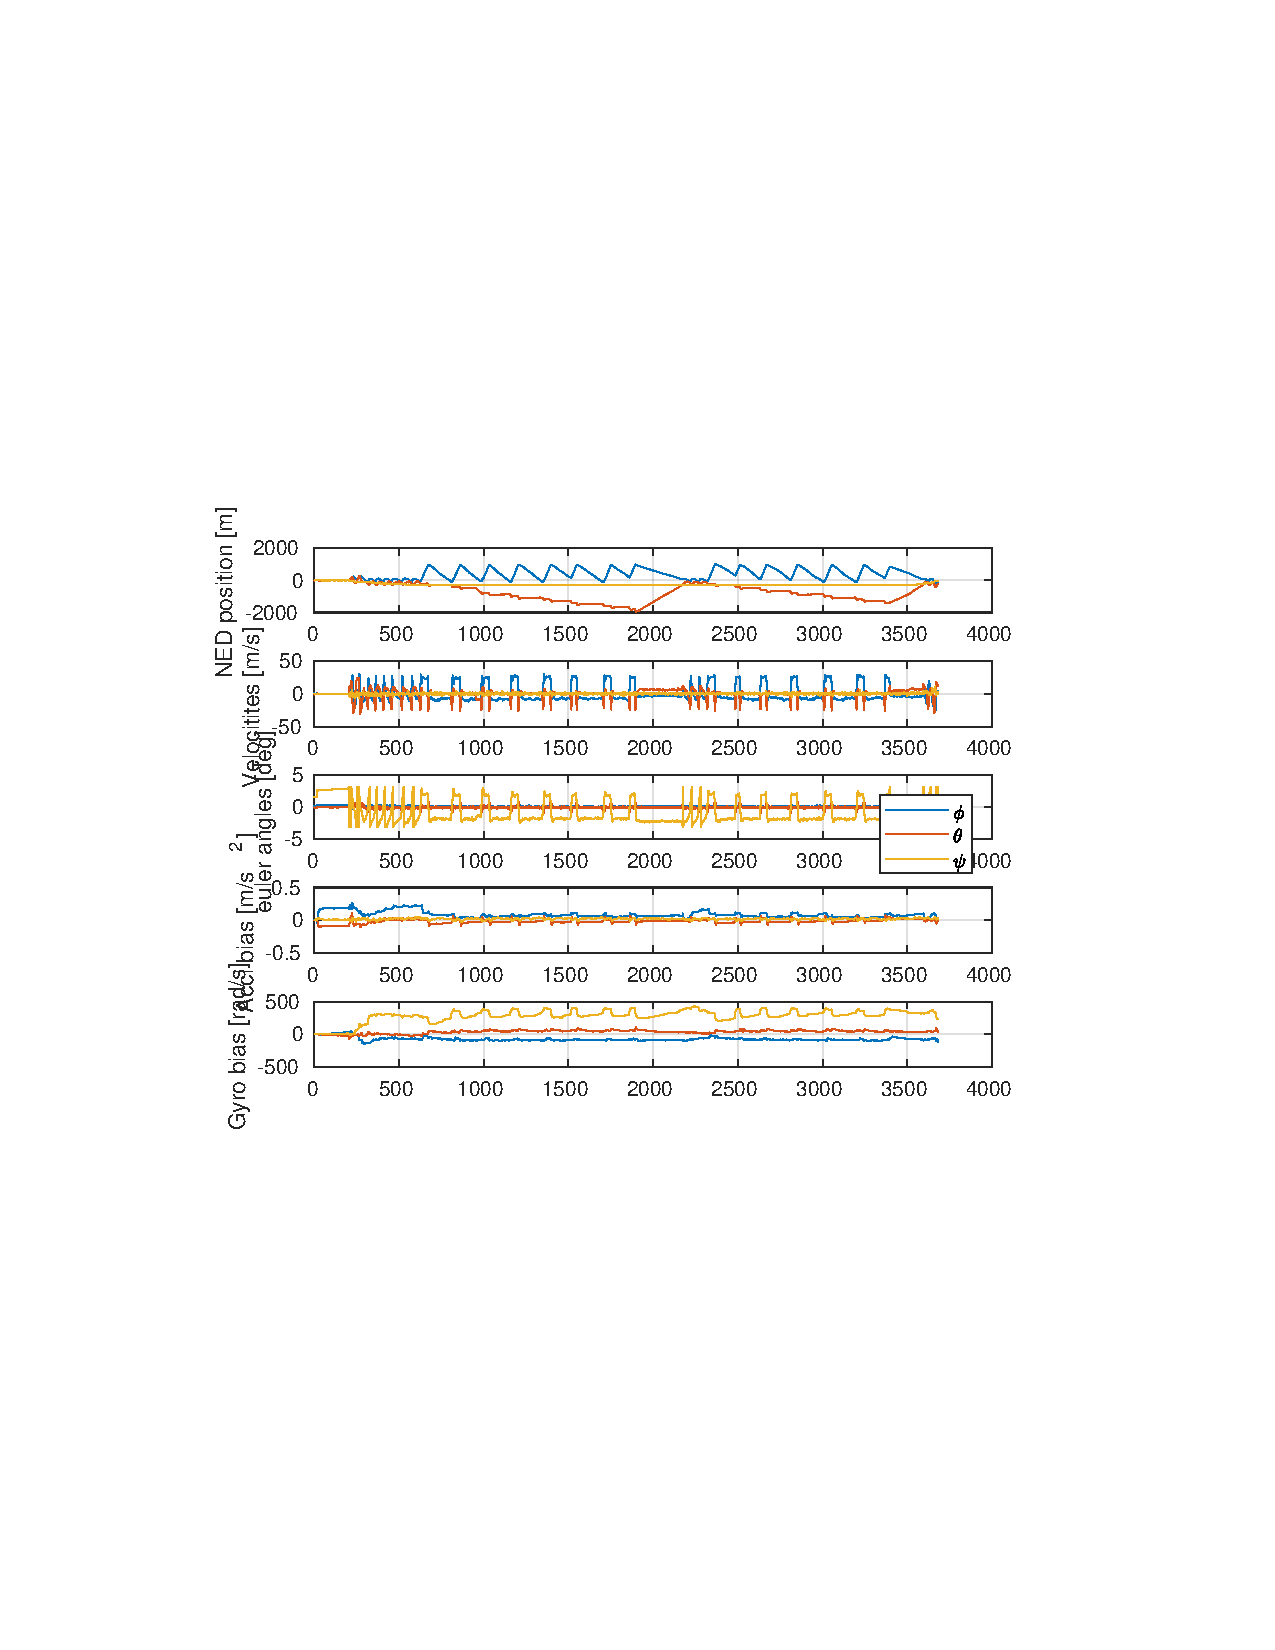
\includegraphics[width=\textwidth]{plots/a2-real-nis}
                \caption{NIS }
                \label{fig:nis_basic}
        \end{subfigure}%
~
        \begin{subfigure}[b]{0.45\textwidth}
                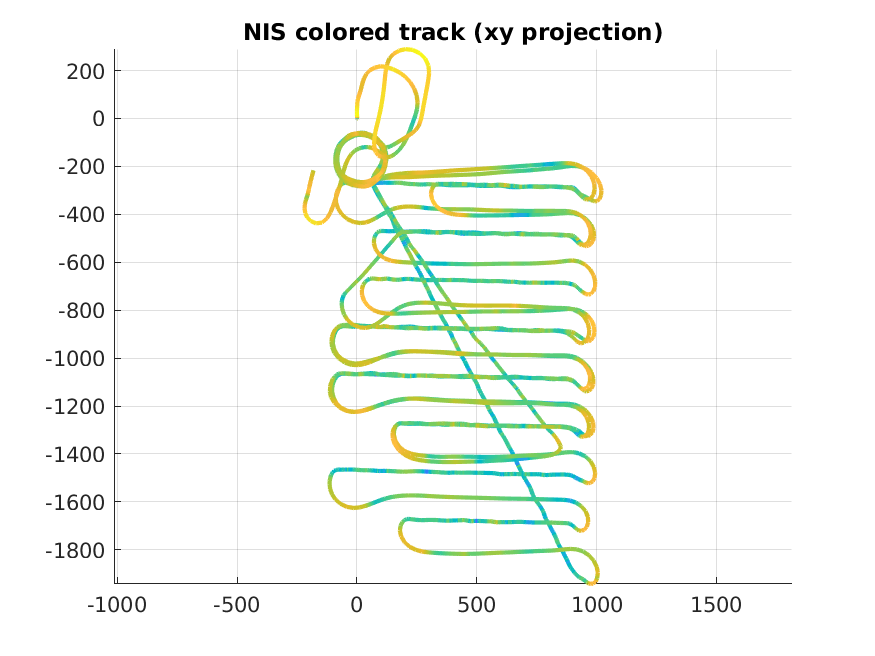
\includegraphics[width=\textwidth]{plots/a2-real-nis-colored-track}
                \caption{NIS colored track}
                \label{fig:nis_colored_track}
        \end{subfigure}
        \caption{Normalized Innovation Squared for the real dataset}
        \label{fig:nis}
\end{figure}
\begin{subequations}
\begin{equation}
q_a = (1.167 \cdot 10^{-3})^2, \\
\end{equation}
\begin{equation}
q_{ab} = (1.5 \cdot 10^{-3})^2, \\
\end{equation}
\begin{equation}
p_{ab} = 0, \\
\end{equation}
\begin{equation}
q_\omega = (2.5 \cdot 10^{-2})^\circ, \\
\end{equation}
\begin{equation}
q_{\omega b} = (2 \cdot 10^{-5})^2, \\
\end{equation}
\begin{equation}
p_{\omega b} = 0, \\
\end{equation}
\end{subequations}




\subsection{Discussion}
This sections contains some thoughts on ESKF from tuning the filter for the simulated and the real dataset.



\subsubsection{Consistency}
When tuning the ESKF we want to achieve high precision, but we also want a consistent filter. In our case we expect increased model errors in the turns due to the non-linear motion, and we want the filters covariance to increase as the model gets less accurate. We superimposed the predicted covariance norm over the XY track to visualize how the filters confidence evolves during the track. As can be seen from \cref{fig:eskf-real-ppred-coloredtrack} the uncertianty increases during the turns as expected. By also superimposing the NIS over the XY track, as seen in \cref{fig:eskf-real-nis-coloredtrack}, we see that our current tuning balance the covariance and innovation well, and there are no significant increase in NIS during turns. 
We also note the large spike in NIS early in \cref{fig:eskf-real-nis-basic} (note the use of logarithm to better visualize the spike). This spike appears at $t=206s$, right as the AUV is catapulted into the air, as such it is natural to expect a sudden increase in innovation.

\subsubsection{Attitude estimation (task 3B)}
The attitude estimation for roll and pitch is very precise which makes sense since they are observable using the IMU due to the constant gravity vector. Yaw is however not possible to observe without additional requirements on the measurements. Without any sensor for measuring global heading (i.e compass) we need to get the heading from the velocity, which we can estimate from the GNSS measurements \textit{if the plane is moving.} If the velocity vector is zero, we have no information about the direction and can not estimate the heading. (i.e lack of suffecient exciation) 

\subsubsection{IMU Mounting errors (task 3C and 4B)}
We tried a few different correction matrices  in the simulated dataset to determine how the correction matrices $S_a$ and $S_g$ affect the performance of our filter. First we rotated the provided $S_a$ and $S_g$ $90^\circ$ in the roll axis and initialized the filter with the same $90^\circ$ offset. We simulated and observed that the filter worked fine with only a minor increase in error (RMSE increased only a few centimeters for position and velocity), except for the expected $90^\circ$ offset in roll attitude compared to ground truth. We then tried to use $S_a = S_g = I$ and observed a substantial increasing in error (RMSE) for all states. RMSE doubled for XY position and almost tripled for XY velocity. It had little effect on the NIS, but the filter became over-confident and NEES was way off.

Mounting errors of the IMU will affect how we define the body frame. In our case we only rely on the attitude of the body frame when transforming the IMU measurement into world frame during prediction, and when updating the estimate using GNSS \textit{due to the leverarm.}. The prediction step would be almost completely unaffected by mounting errors of the IMU as long as the filter is given enough time to converge. As long as the IMU knowns its own orientation it is able to transform the measurements into world frame. The GNSS receiver also depends on the attitude due to the leverarm of the antenna, which is specified in the AUV body frame. The relatively large uncertianty for GNSS does however reduce the impact small mounting errors of the IMU might have. This is why there was no significant increase in error when introdother body frame dependent measurements are useducing large IMU mounting errors. The error would however be larger if more precise GNSS (RTK) or other body frame dependent measurements are used. From this we conclude that the IMU should be mounted correctly (or compenstate for any errors in software), but small errors will not completely break the filter other than an attitude offset in body frame. 

Misalignment of the coordinate axes of the IMU from manufacturing is however a bit worse since we then have correlation between the different axis. Acceleration in one axis will "contaminate" the measurements for the misaligned axes and therefore violate the assumption that the IMU sensor noise is white (we no longer get zero mean due to the added contamination from the misaligned axis). It is therefore important to correct for misalignment errors to get as precise nominal prediction as possible. This is why the error increased when using $S_a = S_g = I$.

We tried the experiment on both the simulated and the real dataset to confirm our reasoning. On the real dataset we do however not have any ground truth to use for error metrics. It is therefore difficult to quantify errors when using another correction matrix. In reality it is diffcult to know if the AUV is affected by small mounting or misalignment errors without somehow aquiring a precise ground truth. Even with ground truth it is difficult to tell if filter errors is caused by wrong correction matrices, by non-optimal tuning or both. 
\section{}
\subsection{Introduction}
\subsubsection{The SLAM Problem}
In any autonomous manouvering situation, be it for a robot, a wheeled vehicle, a flying drone or anything in between, the need for localization is vital.
Localization alone however is only really meaningful in relation to the environment the robot is in.
The SLAM – simultaneous localization and mapping – problem arises then, as the need to simultaneously locate the robot as well as map out its environment.

This problem is naturally non-trivial and has consequently been the topic of extensive research in the last few decades.
There are multiple difficult aspects of the problem that must be solved for a SLAM-system to be successful.
Odometry, i.e. measuring the movement of the robot, map feature/landmark detection, data association as well as estimation and tracking are among the central parts of the SLAM problem that must all be solved.
One of the earliest SLAM solvers, which is the one we will be considering in this assignment is EKF-SLAM, in which an extended Kalman filter fuses together odometric measurements with associated landmark measurements to provide a continuously improved map of the environment and the vehicle position within it.

\subsubsection{EKF-SLAM in Intuitive Terms}
In our problem formulation, we are considering the odometry of the vehicle as given at each timestep, e.g. from an IMU or wheel encoders.
Using this information, typically in the form of velocity estimates or displacement increments, the vehicle can perform dead reckoning to give an indication of where the it has moved over time.
Such a scheme quickly breaks down however, as the inevitably imprecise odometric measurements, when integrated, will give rise to an ever accumulating deviation from the true position of the vehicle. In Kalman filter terms, this corresponds to performing consecutive prediction steps for all time. In order to remove deviations, the natural extension to this scheme is then to include an update step, where the pose, i.e. the position and orientation of the vehicle is updated with information gathered from observing the environment. In that sense, EKF-SLAM is similar to the ESKF, with landmark measurements replacing GNSS for global position updating.

\subsection{Our EKF-SLAM Implementation}
The problem we are considering in this assignment is two-dimensional SLAM, meaning the vehicle is modeled with three degrees of freedom, $x$, $y$ position and orientation $\psi$. In contrast, the ESFK in \ref{sec:a2} was able to represent 6 degrees of freedom. The other major difference is that the state vector in EKF-SLAM contains all the discovered landmarks. We call this state vector the joint pose-landmark vector $\eta_k = \begin{bmatrix} \mathbf{x}_k & \mathbf{m} \end{bmatrix}^{\top}$ as it contains both the pose and all landmarks detected up to the current timestep. In the predict step of the EKF, the pose is compounded (i.e. added in a geometrically meaningful way) with the current odometric vector $\mathbf{u}_k$, in addition to updating the covariance matrix. The update step however is where the action happens. During this step, the EKF does three things. Firstly, it associates new measurements with existing landmarks using Joint Compatibility Branch and Bound, or JCBB for short. Secondly, it calculates an innovation term from the associations that it does an Kalman update step with. Lastly, it augments the state vector with new landmarks – one for each unassociated measurement.



\subsection{Tuning of EKSF-SLAM for simulated dataset} \label{a3-sim-tuning}
We started by tuning the odometry noise $Q$ and measurement noise $R$ by using NEES and NIS to get the initial tuning. NIS and NEES was normalized to get a value between $0$ and $1$ due to the increasing degrees of freedom when adding new landmarks. We used a diagonal $Q$ and tuned the translation and heading independently to improve NEES. The measurement noise $R$ was tuned by attempting to maximize NIS while keeping the entries in $R$ as low as possible. We also created a plot for the position error over time to keep track of the estimation error. We realized that there were a tradeoff between a having a consistent filter (acceptable NIS and NEES) and the estimation error. Trying to improve the NEES resulted in increased error and trying to reduce the estimation error gave us worse NEES and NIS. We decided to prioritize the estimation error when tuning, but also kept an eye on the NEES and NIS to make sure we remained close to the confidene intervals. With our finished tuning we achieved a $82\%$ within NIS CI and $68\%$ within NEES CI, while also keeping the estimaion error reasonably low (less than $0.5m$). The JCBB alphas, $\alpha_1$ and $\alpha_2$, was choosen not to low to avoid making too many wrong associations. Otherwise it was tuned by balancing it with the other parameters while looking at NEES, NIS and estimation error. 

\begin{tcolorbox}[ams align, title={ESKF-SLAM tuning for simulated dataset}]
    Q &= \begin{bmatrix}(5.32*10^{-2})^2 & 0 & 0 \\0 & (5.32*10^{-2})^2 & 0 \\0 & 0 & (1.4*10^{-2})^{2} \end{bmatrix} & R &= \begin{bmatrix}(3.2*10^{-2})^2 & 0 \\0 & (3.2*10^{-2})^2\end{bmatrix} \\
    \alpha_{1} &= 10^{-6} & \alpha_2 &= 10^{-3}
\end{tcolorbox}


\begin{figure}
    \centering
    \begin{subfigure}{0.45\textwidth}
        \includegraphics[width=\textwidth]{plots/a3-sim-nis}
        \caption{NIS}
        \label{fig:a3-sim-nis}
    \end{subfigure}
~
    \begin{subfigure}{0.45\textwidth}
        \includegraphics[width=\textwidth]{plots/a3-sim-nees}
        \caption{NEES}
        \label{fig:results_bg}
    \end{subfigure}
    \begin{subfigure}{0.45\textwidth}
        \includegraphics[width=\textwidth]{plots/a3-sim-error}
        \caption{Error}
        \label{fig:a3-sim-error}
    \end{subfigure}
~
    \begin{subfigure}{0.45\textwidth}
        \includegraphics[width=\textwidth]{plots/a3-sim-results}
        \caption{Track}
        \label{fig:result}
    \end{subfigure}
    \caption{EKF-SLAM results for simulated dataset}
\end{figure}
\subsection{Victoria Park Dataset}
\subsubsection{Computational Performance of EKF-SLAM}
EKF-SLAM has been critizised for a variety of reasons in the literature, and one of the issues often brought up is computational performance as the map grows large. In fact, each timestep of EKF-SLAM has a computational complexity of $\mathcal{O}(n^2)$ in the number of detected landmarks. \cite{divideandconq} Our implementation, when tuned to provoke lots of landmark detections (around 800) resulted in the update step of the Kalman filter taking quadratic time, as shown in figure \ref{fig:update_time_landmarks}. These results show that in large environments, EKF-SLAM alone fails to meet the time-requirements for online SLAM.
\begin{figure}[H]
\centering
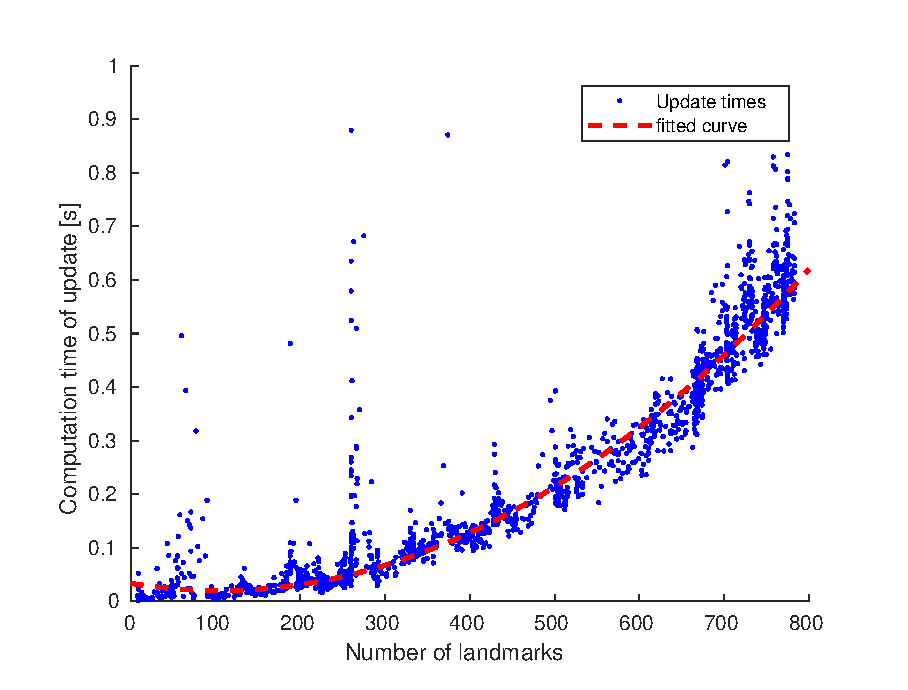
\includegraphics[width=0.7\textwidth]{plots/a3/update-time-vs-landmarks}
\caption{Update time vs landmarks}
\label{fig:update_time_landmarks}
\end{figure}



\subsubsection{Computational Performance of EKF-SLAM}
EKF-SLAM has been critizised for a variety of reasons in the literature, and one of the issues often brought up is computational performance as the map grows. Keeping the computation time down is of paramount importance in the online SLAM problem where delayed updates are not acceptable. In fact, each timestep of EKF-SLAM has a computational complexity of $\mathcal{O}(n^2)$ in the number of detected landmarks\cite{divideandconq}, something our implementation confirms. When tuned to provoke lots of landmark detections (around 800), the update step of the Kalman filter takes quadratic time, as shown in figure \ref{fig:update_time_landmarks}. These results show that in large environments, EKF-SLAM alone fails to meet the time-requirements for online SLAM.
\begin{figure}
    \centering
    \begin{subfigure}{0.45\textwidth}
        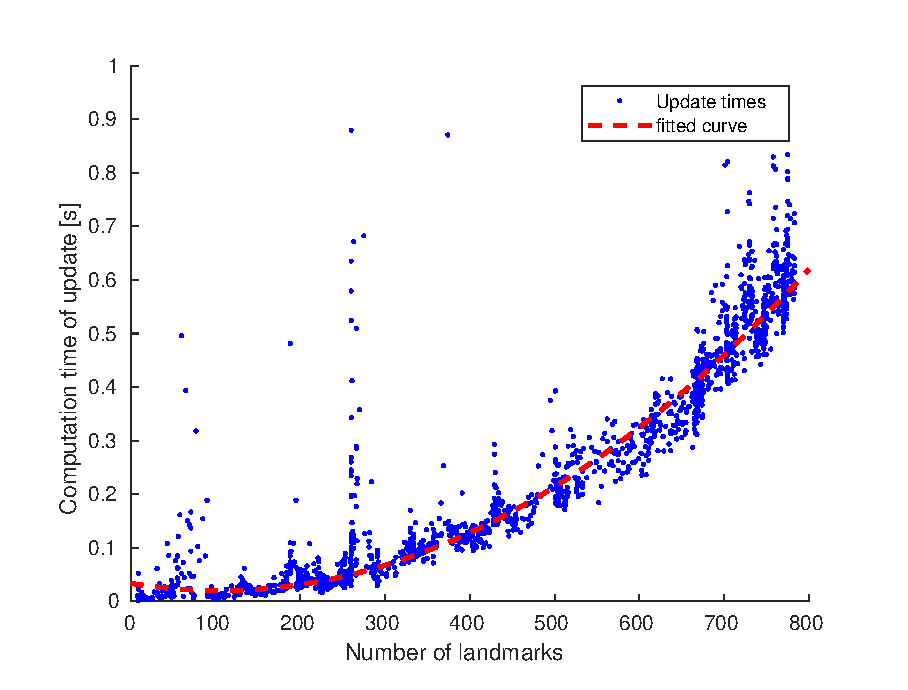
\includegraphics[width=\textwidth]{plots/a3/update-time-vs-landmarks}
        \caption{Update time vs landmarks}
        \label{fig:update_time_landmarks}
    \end{subfigure}%
~
    \begin{subfigure}{0.45\textwidth}
        \includegraphics[width=\textwidth]{plots/a3-real-results-bg}
        \caption{Trajectory overlayed Google Maps}
        \label{fig:results_bg}
    \end{subfigure}
\end{figure}

\subsubsection{Measurement Clutter}
After a successful run of the EKF-SLAM algorithm on the Victoria Park dataset, we typically find around 300 landmarks. For this reason, we have speculated that not all these landmarks correspond to actual trees, even though that is what they are supposed to represent. One of the reasons for this is landmarks being doubly registered due to the JCBB algorithm not making the proper associations. But another reason that must not be overlooked is the effect of clutter in the measurement data. The laser data in the dataset has been processed to only contain measurements that match a certain tree-profile\cite{victoria}, however no classification algorithm is perfect and we speculate that a lot of the measurements are spurious and should be regarded as clutter. This partly stems from the fact that a lot of the detected landmarks happen to appear inside the six-lane intersection to the east of Victoria Park, as can be seen in figure \ref{fig:results_bg}. In our experiments, the effect of clutter has not been significant, and spuriously detected landmarks have not had a noticeable impact on SLAM performance. It might however become problematic for longer operation times and larger maps. Keeping the number of landmarks down is essential to successfully apply EKF-SLAM in an online situation. In addition, wrongly registered landmarks might lead to spurious associations in the future and ultimately worsen the tracking performance. In our implementation, all unassociated measurements are initialized as new landmarks and never face the possibility of removal, there are however techniques to remove landmarks which have low probability of corresponding to an actual real life feature. One possibility would be to employ something akin to the IPDA mentioned in \ref{sec:a1} since it has a concept of target existance that in a SLAM context could be used to discriminate false landmarks.

\subsubsection{Choice of JCBB CI Bounds with Implication on Robustness}
The JCBB algorithm operates with two confidence intervals, one for joint and one for individual compatibility. The Mahalonobis distances of both joint and individual compatibility are gated with these confidence intervals to determine whether to move on with a given hypothesis.\cite{jcbb} In the Victoria Park dataset, we found that the choice of large confidence intervals ($\alpha_1 = 10^{-5}$ and $\alpha_2 = 10^{-3}$ for joint and individual respectively) gave perfectly satisfactory association speed on the dataset, however when EKF-SLAM was rerun on the generated map with a slight offset in orientation of $6^\circ$ (such a situation could appear naturally from disturbances such temporary loss of sensor data), the JCBB algorithm wound up in an almost complete stall after a few hundred timesteps, likely because all hypothesis were regarded as more equally likely due to the offset, making the algorithm unable to reduce the search tree and single out the best association in reasonable time. Choosing tighter confidence intervals on the other hand, with $\alpha = 0.1$ for both joint and individual, many more associations were gated out and hence only the most promising hypotheses were considered, ultimately leading to reasonable execution times. In the end, this made the rerun on the previously built map perfectly possible with no significant slow-down. This result shows how the choice of these confidence intervals is detrimental to the robustness of EKF-SLAM and crucial for online SLAM as a small disturbance can cause the JCBB algorithm to fail to find associations within reasonable time.




\section{Conclusion}
During this course we have used the IMM-PDAF approach for tracking a boat through tight turns, using only a radar mounted on a nearby ship. We have also developed an ESKF that is able to estimate 6 degrees of freedom using inertial navigation. We have also implemented the EKF-SLAM approach for solving the \texttt{Simultaneous Localization And Mapping} problem using a lidar scanner and odometry measurement. Throughout the course we have used metrics such as NEES and NIS to quantify our implementations ability to be consistent, while also tuning our filters to be precise.

\printbibliography
\end{document}

